
\subsection{Integration auf Präsentationsebene}

für Client-Tier

\subsubsection{Client-App-orientierte Integration}

Von unterschiedlichen Anwendungen in eine einheitliche Client-Oberfläche. Integration der EC-Karte und Checkout über Payment Provider. Vorteil ist die rasche Realisierung mit Widgets. Nachteil sind die Abhängigkeiten

\begin{itemize}
    \item UI-Rahmen App
    \item Widgets
    \item Identity-Provider für Login
    \item Payment-Provider für Zahlungsprozess
\end{itemize}

\subsubsection{Portalorientierte Integration}
thematisch ausgerichtete Portallösung. Bsp. Mitarbeiterportal. Primär ein SSO (Single Sign-on). Vorteil Stakeholder muss nur einen Zugangslink mit Zugangsinformationen merken.

\begin{itemize}
    \item Lieferantenportal
    \item Kundenportal
    \item Mitarbeiterportal
\end{itemize}

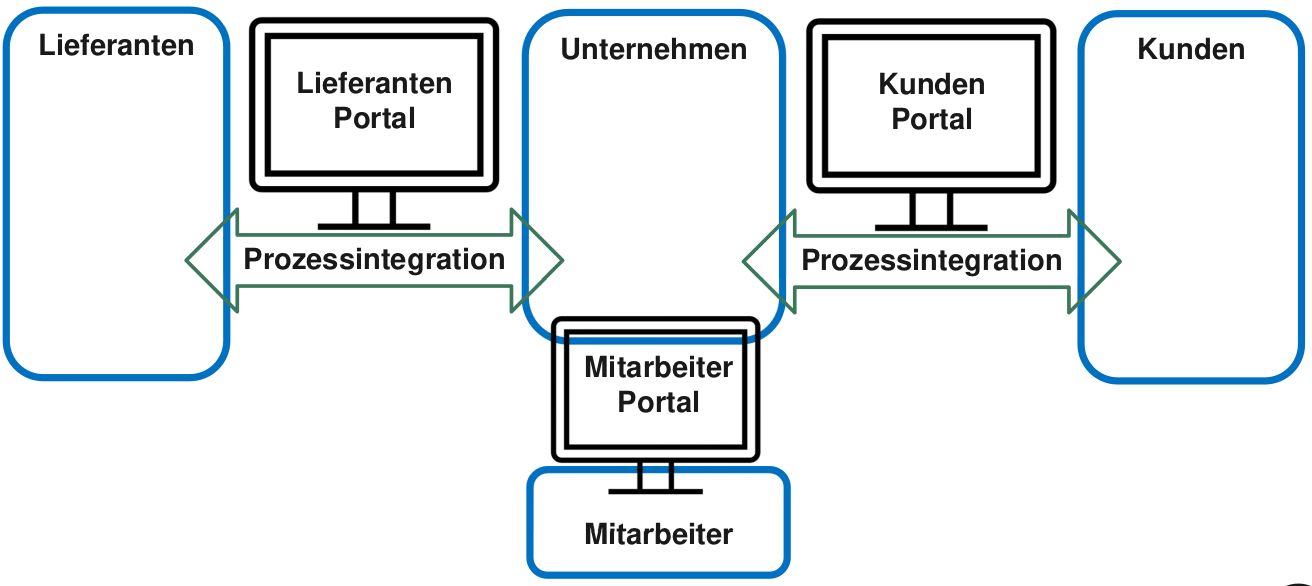
\includegraphics[width=\linewidth]{integration-presentation-portal.png}

\subsubsection{Geschäftsprozessorientierte Integration}

mittels WfMS (Workflow Management System). Vorteil Hohes Einsparungspotenzial bei stark strukturierten, komplexen und häufig ausgeführten Workflows

\begin{itemize}
    \item Funktion einer Middleware
    \item Integriert in einer Fachapplikation
    \item dedizierten WfMS
\end{itemize}
\vspace{10pt}
\textbf{WfMC Referenzmodell}

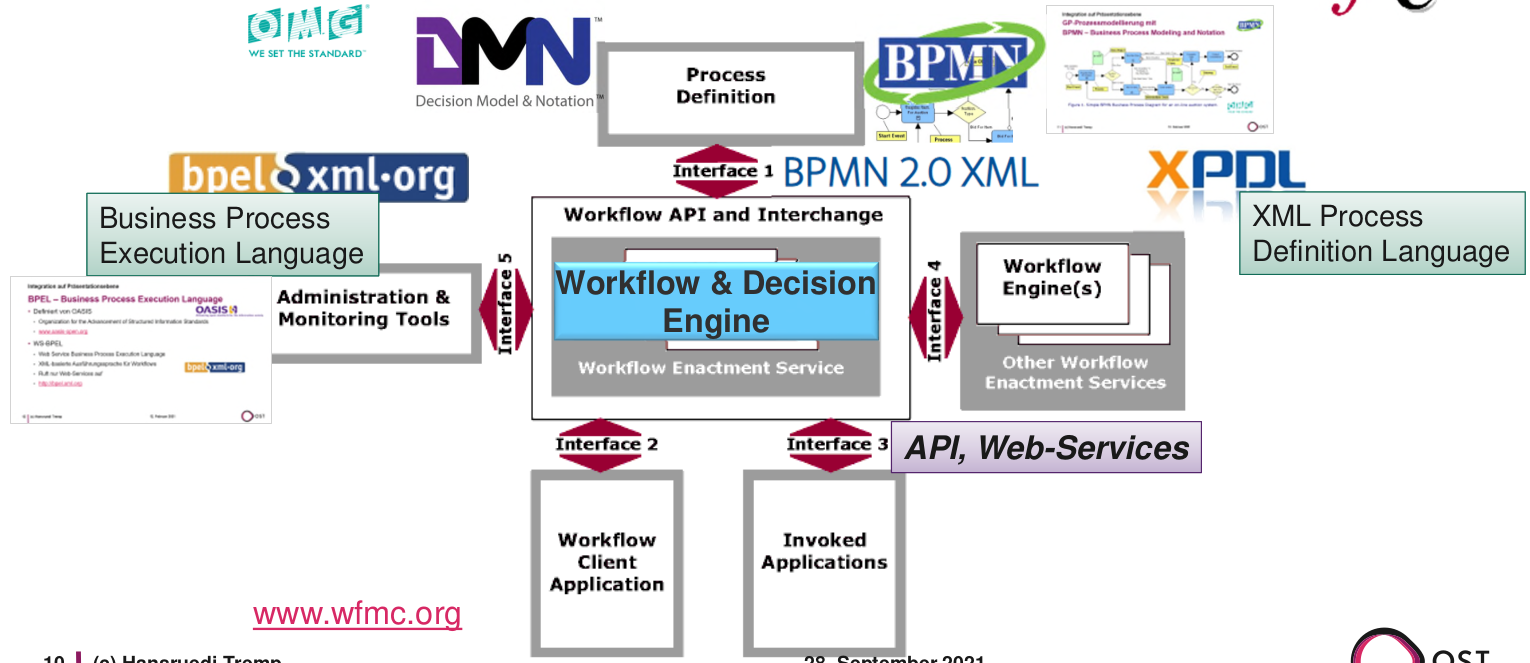
\includegraphics[width=\linewidth]{integration-wfmc-workflow.png} \\

\textcolor{blue}{Process Definition}

GP-Prozessmodellierung mit BPMN (Business Process Modeling and Notation)

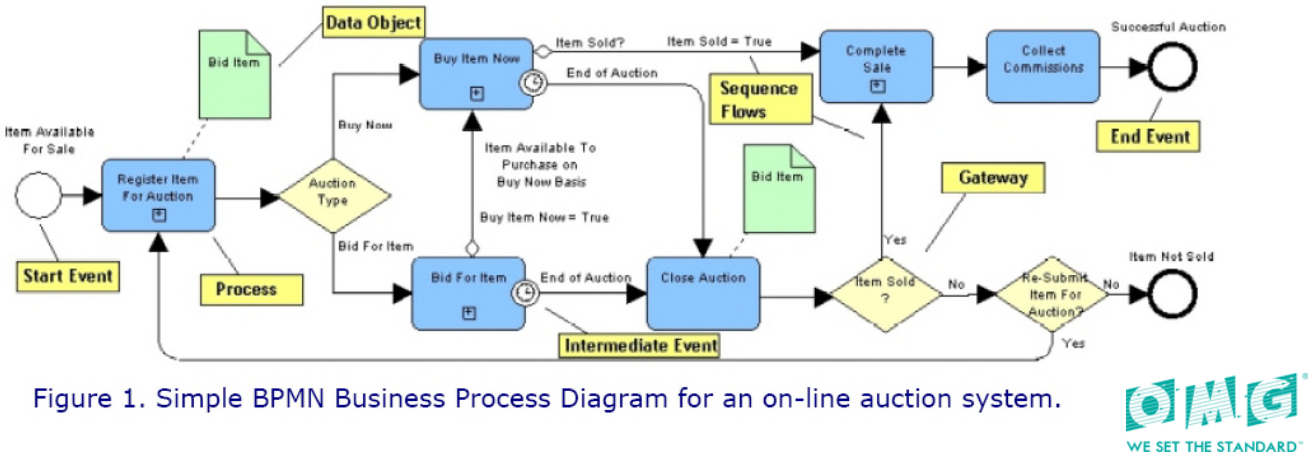
\includegraphics[width=\linewidth]{integration-omg-bpmn.png}

Funktionsübersicht

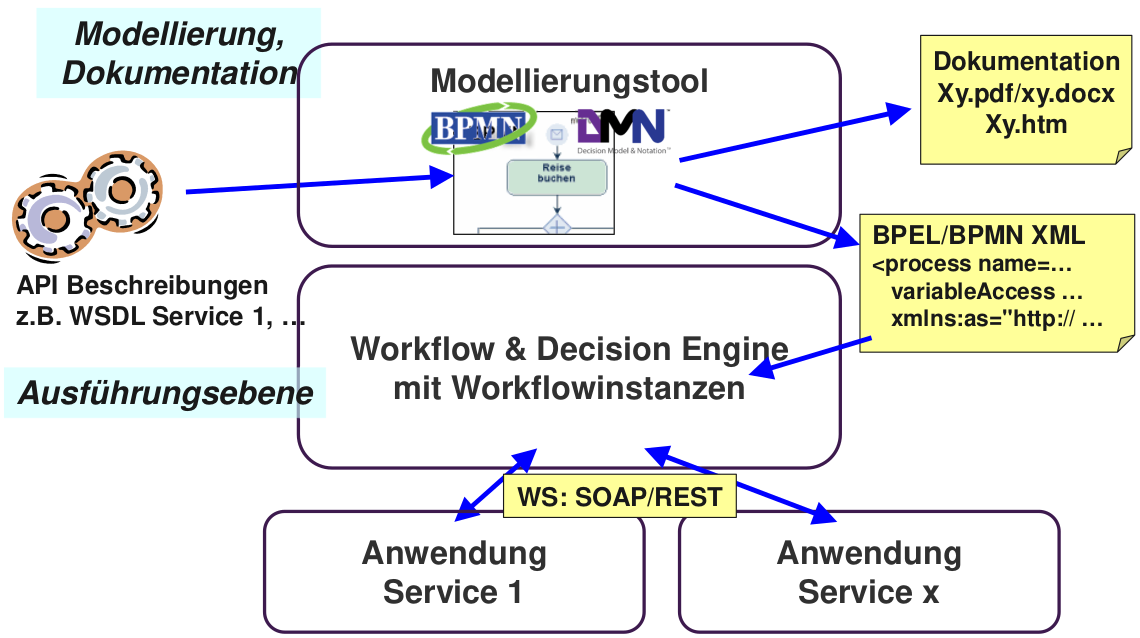
\includegraphics[width=\linewidth]{integration-omg-functions.png} \\

\textbf{WfMS Referenzarchitektur}

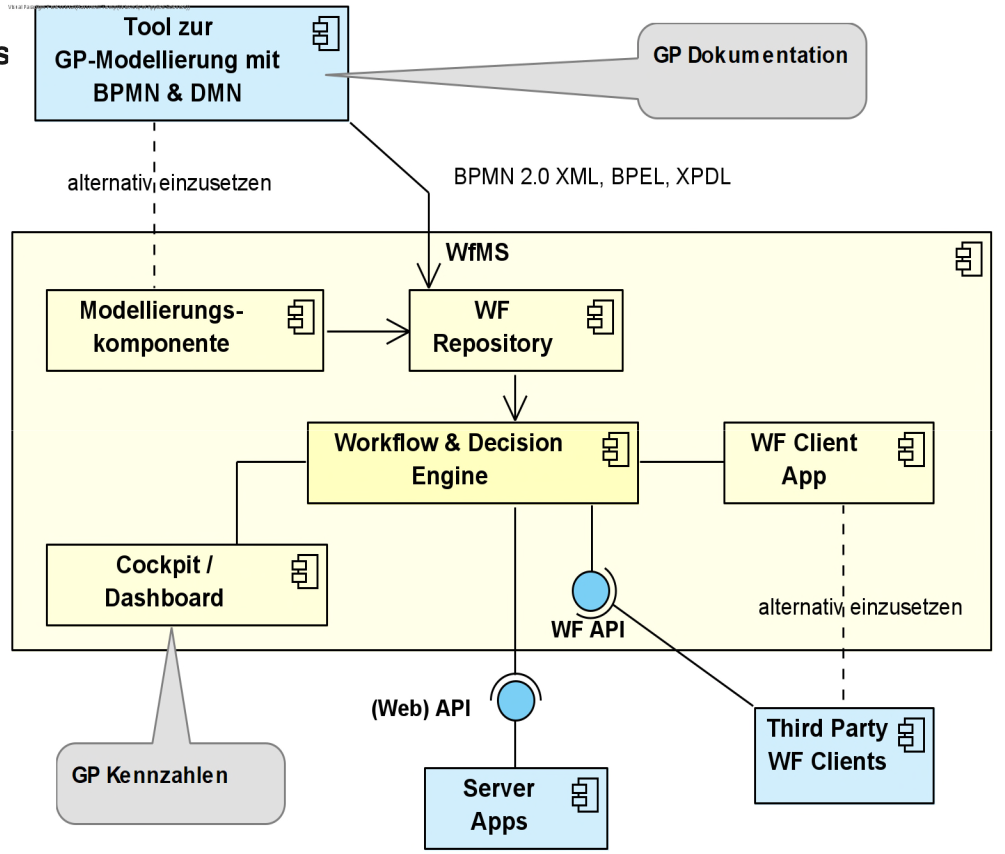
\includegraphics[width=\linewidth]{integration-wfms-workflow.png}

